%\documentclass[10pt,twocolumn,letterpaper,draft]{article}
\documentclass[10pt,letterpaper]{article}

% 使用中文宏包
\usepackage[UTF8]{ctex}
\usepackage{graphicx} %插入图片的宏包
\usepackage{float} %设置图片浮动位置的宏包
\usepackage{subfigure} %插入多图时用子图显示的宏包

\usepackage[strings]{underscore}
\usepackage{times}
\usepackage{epsfig}
\usepackage{amsmath}
\usepackage{amssymb}
\usepackage{overpic}
\usepackage{listings}
\usepackage{color}
\usepackage{enumitem}
\setenumerate[1]{itemsep=0pt,partopsep=0pt,parsep=\parskip,topsep=5pt}
\setitemize[1]{itemsep=0pt,partopsep=0pt,parsep=\parskip,topsep=5pt}
\setdescription{itemsep=0pt,partopsep=0pt,parsep=\parskip,topsep=5pt}

\definecolor{mygreen}{rgb}{0,0.6,0}
\definecolor{mygray}{rgb}{0.5,0.5,0.5}
\definecolor{mymauve}{rgb}{0.58,0,0.82}
\lstset{ %
  backgroundcolor=\color{white},   % choose the background color
  basicstyle=\footnotesize,        % size of fonts used for the code
  breaklines=true,                 % automatic line breaking only at whitespace
  captionpos=b,                    % sets the caption-position to bottom
  commentstyle=\color{mygreen},    % comment style
  escapeinside={\%*}{*)},          % if you want to add LaTeX within your code
  keywordstyle=\color{blue},       % keyword style
  stringstyle=\color{mymauve},     % string literal style
}

% Include other packages here, before hyperref.

% If you comment hyperref and then uncomment it, you should delete
% egpaper.aux before re-running latex.  (Or just hit 'q' on the first latex
% run, let it finish, and you should be clear).
\usepackage[pagebackref=true,breaklinks=true,letterpaper=true,colorlinks,bookmarks=false]{hyperref}


\def\httilde{\mbox{\tt\raisebox{-.5ex}{\symbol{126}}}}

\newcommand{\cmm}[1]{\textcolor[rgb]{0,0.6,0}{CMM: #1}}
\newcommand{\todo}[1]{{\textcolor{red}{\bf [#1]}}}
\newcommand{\alert}[1]{\textcolor[rgb]{.6,0,0}{#1}}

\newcommand{\IT}{IT\cite{98pami/Itti}}
\newcommand{\MZ}{MZ\cite{03ACMMM/Ma_Contrast-based}}
\newcommand{\GB}{GB\cite{conf/nips/HarelKP06}}
\newcommand{\SR}{SR\cite{07cvpr/hou_SpectralResidual}}
\newcommand{\FT}{FT\cite{09cvpr/Achanta_FTSaliency}}
\newcommand{\CA}{CA\cite{10cvpr/goferman_context}}
\newcommand{\LC}{LC\cite{06acmmm/ZhaiS_spatiotemporal}}
\newcommand{\AC}{AC\cite{08cvs/achanta_salient}}
\newcommand{\HC}{HC-maps }
\newcommand{\RC}{RC-maps }
\newcommand{\Lab}{$L^*a^*b^*$}
\newcommand{\mypara}[1]{\paragraph{#1.}}

\graphicspath{{figures/}}


\setcounter{page}{1}

\begin{document}


%%%%%%%%% TITLE

\title{《信息论基础》\cite{cover2005信息论基础} 笔记}

\author{纳文琪$^{1}$}

\maketitle


\section{熵、相对熵与互信息}
\subsection{熵}
\paragraph{熵} 是随机变量不确定度的度量,离散型随机变量X的熵定义为:\\
\begin{equation}
	\begin{split}
		H(X) &= -\sum_{x\in X} p(x)\log p(x) \\
		&= -E \log{p(x)}
	\end{split}
\end{equation}
熵不依赖于X的实际取值,值依赖于其概率分布。性质:
\begin{equation}
	H(X) \geq 0
\end{equation}


\subsection{联合熵与条件熵}

\paragraph{联合熵} 与联合分布相对应,定义为:\\
\begin{equation}
	\begin{split}
		H(X,Y) &= -\sum_{x \in X} \sum_{y \in Y} p(x,y)\log {p(x,y)} \\
		&= -E \log{p(x,y)}
	\end{split}
\end{equation}

\paragraph{条件熵} 与条件概率对应,定义为: \\
\begin{equation}
	\begin{split}
		H(Y|X) &= \sum_{x \in X} p(x) H(Y|X=x) \\
		&= E \log{p(Y|X)}
	\end{split}
\end{equation}

\paragraph{链式法则} 定位为:\\
\begin{equation}
	H(X,Y) = H(X) + H(Y|X)
\end{equation}
其含义是:一对随机变量的熵等于其中一个随机变量的熵加上另一个随机变量的条件熵。

\paragraph{熵的链式法则}
\begin{equation}
	H(X_1,X_2,\cdots, X_n) = \sum_{i=1}^n H(X_i|X_{i-1}, \cdots, X_1)
\end{equation}

\subsection{相对熵与互信息}
\paragraph{相对熵(relative entropy, KL距离)}是两个随机分布之间距离的度量,也就是说它表示两个随机变量之间的距离。定义为:\\
\begin{equation}
	\begin{split}
		D(p \parallel q) &= -\sum_{x\in X} p(x)\log{\frac{p(x)}{q(x)}} \\
		&= E \log{\frac{p(X)}{q(X)}}
	\end{split}
\end{equation}
相对熵总是非负的,且当且仅当$p=q$时为零。它不对称,也不满足三角不等式,但将其视作分布之间的“距离”往往会很有用。
\paragraph{自信息} ?
\paragraph{互信息} 是一个随机变量包含另一个随机变量信息量的度量。定义为:\\
\begin{equation}
	\begin{split}
		I(X;Y) &= -\sum_{x \in X} \sum_{y \in Y} p(x,y)\log {\frac{p(x,y)}{p(x)p(y)}}\\
		&= D(p(x,y) \parallel p(x)p(y)) \\
		&= H(X) - H(X|Y) \\
		&= H(Y) - H(Y|X)
	\end{split}
\end{equation}
互信息I(X;Y)是在给定Y的知识的条件下X的不确定度(熵)的缩减量;而且,X含有Y的信息量等同于Y含有X的信息量。
\begin{figure}[H] %H为当前位置,!htb为忽略美学标准,htbp为浮动图形
	\centering %图片居中
	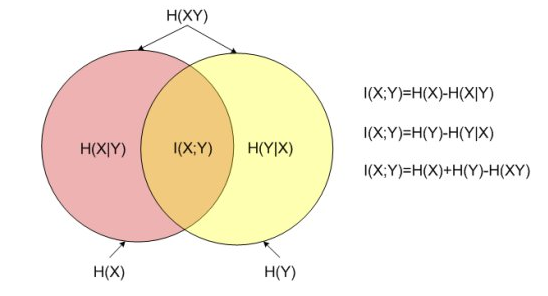
\includegraphics[width=0.7\textwidth]{../images/shang_huxinxi.png} %插入图片,[]中设置图片大小,{}中是图片文件名
	\caption{熵与互信息的关系} %最终文档中希望显示的图片标题
	\label{Fig.main2} %用于文内引用的标签
\end{figure}

\paragraph{互信息的链式法则}
\begin{equation}
	I(X_1,X_2,\cdots, X_n;Y) = \sum_{i=1}^n I(X_i;Y|X_{i-1}, \cdots, X_1 )
\end{equation}

\paragraph{条件相对熵}
\paragraph{相对熵的链式法则}

\section{数据压缩}
\paragraph{信源编码} 关于随机变量X的信源编码C,是从X的取值空间X到$D^*$的一个映射,其中$D^*$表示D元字幕表上有限长度的字符串所构成的集合。
\paragraph{信源编码的期望长度}
\begin{equation}
	L(C) = E[l(x)]
\end{equation}
其中$l(x)$是$x$的码字长度。

\section{信道容量}
\paragraph{离散信道} 是由输入字母表X、输出字母表Y和概率转移矩阵$p(y|x)$构成的系统,其中$p(y|x)$表示发送字符$x$的条件下收到字符$y$的概率。
\paragraph{离散无记忆信道(DMC)} 如果离散信道输出的概率分布仅依赖于它所对应的输入,而与先前信道的输入或输出条件独立,则称信道是独立的。
\paragraph{DMC的信道容量} 定义为:
\begin{equation}
	C = \max_{p(x)}I(X;Y)
\end{equation}

\subsection{信道容量的几个例子}
\paragraph{无噪声二元信道} 任何一个传输的比特都能被无误差第接收到。信道容量$C=1$
\paragraph{二元对称信道(BSC)} 这个信道的输入字符以概率$p$互补。其信道容量是$C=1-H(p)$
\paragraph{码率} 如果输入序列的长度为$k$,而输出序列的长度为$n$,则码率为:
\begin{equation}
	r=\frac{k}{n},(r<1)
\end{equation}

\paragraph{消息(Word)}是一个字符序列。
\paragraph{码字(Codewords)} 是由消息组成的向量。(?)
\paragraph{码(Code)} 是一组码字的集合。
\paragraph{信道的(M,n)码}指的是将M个消息生成长度为n的码字的一种编码。
\paragraph{(M,n)码的码率} 为:
\begin{equation}
	R=\frac{\log M}{n}
\end{equation}
单位为“bits/传输”。
\paragraph{Example 3.4}  The code $C = {00000, 10100, 11110, 11001}$ is a block code of block length n = 5. Here q = 2(binary code), n = 5 and therefore, k = 2 and M = 4. Since there 4 codewords in the code, it can be used to represent two bit binary numbers. Such as:
\begin{center}
	Uncoded bits	Codewords \\
	    00  		00000 \\
		01			10100 \\
		10			11110 \\
		11			11001
\end{center}
\paragraph{汉明距离} 它表示两个(相同长度)字对应位不同的数量。
\paragraph{线性码} 具有以下属性:
\begin{itemize}
	\item 两个码字的和同样属于码
	\item 全0消息也是一个码字
	\item 两个码字的最小汉明距离与任何非零码字的最小权重相等,即$d^∗ = w^∗$
\end{itemize}

\paragraph{信道编码定理(香农第二定理)} 对于DMC,小于信道容量$C$的所有码率都是可达的。具体来说,对任意码率$R<C$,存在一个$(2^{nR},n)$码序列,它的最大误差概率为$\lambda^{(n)} \rightarrow 0$。

\paragraph{重复码(Repetition Code)}中每个输入被简单重复$n$次,n为奇数。例如,n=3时,有: \\
$ 0 \rightarrow 000, 1 \rightarrow 111 $。它的码率为: $r=\frac{1}{n}$。其解码策略是多数解码(Majority Decoding),即当接收到的n个比特信息中0的个数大于1的个数的时候,就解码为0,反之亦然。

\paragraph{信道容量定理} 频率为$W Hz$,被谱密度为$N_0/2$的附加白噪声(AWGN)干扰的连续信道的信道容量是:
\begin{equation}
	C = W\log_2(1+\frac{P}{N_0W} ) bits/second
\end{equation}
P是平均传输功率。






\subsection{其他}
\paragraph{香农限制(Shannon Limit)}

\paragraph{Bandwidth Eifficiency Diagram}

\paragraph{域} 是一个可以在其上进行加法、减法、乘法和除法运算而结果不会超出域的集合。
\paragraph{有限域} 是仅含有限个元素的域。有限域中元素的个数称为有限域的阶。每个有限域的阶必为素数的幂,即有限域的阶可表示为$p^n$(p是素数、n是正整数),该有限域通常称为Galois域(Galois Fields),记为$GF(p^n)$。





\bibliographystyle{ieeepes}
\bibliography{../Saliency}
\end{document}



























































